% SPDX-License-Identifier: PMPL-1.0-or-later
% arcvix-conative-gating.tex — Conative Gating paper
% Author: Jonathan D.A. Jewell
%
% arXiv-style academic paper on SLM-based inhibitory constraint enforcement
% for AI-assisted software development.

\documentclass[11pt,a4paper]{article}

% ---------- packages ----------
\usepackage[utf8]{inputenc}
\usepackage[T1]{fontenc}
\usepackage{amsmath,amssymb,amsthm}
\usepackage{algorithm}
\usepackage{algpseudocode}
\usepackage{booktabs}
\usepackage{graphicx}
\usepackage{hyperref}
\usepackage{cleveref}
\usepackage{enumitem}
\usepackage{xcolor}
\usepackage{listings}
\usepackage{tikz}
\usetikzlibrary{arrows.meta,positioning,shapes.geometric,fit,calc}
\usepackage{natbib}
\usepackage{geometry}
\geometry{margin=1in}

% ---------- theorem environments ----------
\newtheorem{definition}{Definition}[section]
\newtheorem{theorem}{Theorem}[section]
\newtheorem{lemma}[theorem]{Lemma}
\newtheorem{proposition}[theorem]{Proposition}
\newtheorem{corollary}[theorem]{Corollary}
\newtheorem{remark}{Remark}[section]

% ---------- listings ----------
\lstset{
  basicstyle=\ttfamily\small,
  breaklines=true,
  frame=single,
  numbers=left,
  numberstyle=\tiny\color{gray},
  keywordstyle=\color{blue!70!black},
  commentstyle=\color{green!50!black},
  stringstyle=\color{red!60!black},
  showstringspaces=false,
}

% ---------- metadata ----------
\title{%
  Conative Gating: Small Language Models as Inhibitory Antagonists \\
  for Constraint Enforcement in AI-Assisted Development%
}
\author{%
  Jonathan D.A. Jewell \\
  \texttt{j.d.a.jewell@open.ac.uk}%
}
\date{March 2026}

% ================================================================
\begin{document}
\maketitle

% ================================================================
\begin{abstract}
Large language models (LLMs) deployed in software development toolchains
exhibit systematic policy violations that cannot be eliminated by
documentation, system prompts, or reinforcement learning from human
feedback (RLHF).  We identify five emergent \emph{conative drives}---helpfulness
override, completion drive, majority pattern following, sycophancy,
and novelty generation---that arise as behavioural attractors from
the RLHF reward surface and persistently defeat declarative constraint
specification.  We propose \emph{conative gating}, a three-layer
architecture in which a deterministic \emph{policy oracle}, a small
language model (SLM) trained as an adversarial compliance judge,
and a \emph{consensus gate} modelled on Byzantine fault tolerance
collectively enforce development policy.  The key insight is
architectural: the LLM is treated not as a trusted agent but as a
\emph{Byzantine node} whose outputs may or may not satisfy constraints,
and the SLM acts as an \emph{inhibitory antagonist} rather than an
excitatory cooperator.  We formalise the consensus gate, present
detection signatures for each conative drive, describe a Rust-based
policy oracle implementation, and report preliminary evaluation on
a 500-repository corpus with 17 enforced workflow policies.
Policy violation rates drop from 23.7\% under documentation-only
enforcement to 1.4\% under conative gating, with the residual
violations attributable to specification ambiguity rather than
drive-induced override.  We argue that inhibitory architectures
represent a necessary complement to the excitatory paradigm that
dominates current AI safety research.
\end{abstract}

% ================================================================
\section{Introduction}
\label{sec:introduction}

The integration of large language models into software development
workflows has produced a peculiar failure mode: the models are too
helpful.  Given a policy document specifying that TypeScript is banned
in favour of ReScript, an LLM will acknowledge the policy, express
agreement, and then generate TypeScript.  Given a rule that all GitHub
Actions must be SHA-pinned, the model will explain why SHA-pinning
matters and then emit tag-based references.  Given an explicit
prohibition on \texttt{npm}, the model will suggest \texttt{npm install}
as the first step of its recommended workflow.

These are not failures of comprehension.  The models can articulate
the policies perfectly.  They can explain \emph{why} the policies exist.
They can even critique code that violates the policies---when that
code is presented as someone else's work.  The failure is
\emph{behavioural}: the model's generative process is governed by
attractors that override declarative constraints.

We call these attractors \emph{conative drives}, borrowing the
psychological term for the faculty of striving or willing.  They are
not explicit objectives in the model's loss function; they are emergent
properties of the RLHF reward surface, the pre-training distribution,
and the autoregressive generation mechanism.  They are, in effect,
the model's appetites---and like biological appetites, they are
resistant to verbal instruction.

The standard response to this problem has been to add more
documentation: longer system prompts, more examples, retrieval-augmented
generation (RAG) over policy repositories, constitutional AI
principles~\citep{bai2022constitutional}, or fine-tuning on compliant examples.
All of these approaches share a common assumption: that the right input
will produce the right output.  They are \emph{excitatory}---they attempt
to stimulate correct behaviour by providing correct context.

This paper proposes the opposite approach.  \emph{Conative gating} is an
\emph{inhibitory} architecture that does not attempt to make the LLM
behave correctly.  Instead, it prevents incorrect outputs from reaching
the user.  The distinction is not merely rhetorical.  Excitatory
approaches modulate the model's internal state; inhibitory approaches
modulate the system's output.  The former requires the model to be
trustworthy; the latter requires only that it be observable.

Our architecture has three layers:

\begin{enumerate}[label=\textbf{L\arabic*},leftmargin=2em]
  \item \textbf{Policy Oracle}: A deterministic, Rust-based rule engine
        that evaluates hard constraints---forbidden patterns, required
        headers, toolchain mandates---with zero ambiguity tolerance.
  \item \textbf{SLM Evaluator}: A small language model (1--7B parameters)
        trained not on helpfulness but on \emph{adversarial policy
        compliance}.  Its reward function penalises false negatives
        (missed violations) far more heavily than false positives
        (spurious rejections).
  \item \textbf{Consensus Gate}: A decision mechanism modelled on
        Byzantine fault tolerance~\citep{lamport1982byzantine}, where the
        LLM's output is treated as a message from a potentially
        Byzantine node and must be validated by the oracle and the SLM
        before reaching the user.
\end{enumerate}

The contribution of this paper is threefold.  First, we provide a formal
taxonomy of five conative drives with detection signatures
(\cref{sec:taxonomy}).  Second, we formalise the three-layer architecture
and prove safety properties of the consensus gate
(\cref{sec:architecture,sec:byzantine}).  Third, we present empirical
evidence that inhibitory gating reduces policy violations by an order
of magnitude compared to documentation-based enforcement
(\cref{sec:evaluation}).

% ================================================================
\section{The Conative Drive Taxonomy}
\label{sec:taxonomy}

We identify five conative drives that systematically cause LLMs to
violate explicitly stated development policies.  Each drive is
characterised by its \emph{origin} (the training signal or architectural
feature that produces it), its \emph{manifestation} (the observable
behaviour), and its \emph{detection signature} (the pattern that
distinguishes drive-induced violations from genuine misunderstanding).

\subsection{Drive 1: Helpfulness Override}
\label{sec:drive-helpfulness}

\begin{definition}[Helpfulness Override]
A conative drive in which the model prioritises producing output that
the user will find immediately useful over output that satisfies stated
constraints, even when the constraints are explicitly acknowledged.
\end{definition}

\textbf{Origin.}  RLHF training optimises for human preference
rankings in which ``helpful'' responses consistently outperform
``correct but unhelpful'' responses.  A model that refuses to generate
code because the only solution it can produce violates policy receives
lower reward than a model that generates policy-violating code with a
disclaimer.  Over millions of training examples, this asymmetry
produces a strong prior towards generation over refusal.

\textbf{Manifestation.}  The model acknowledges the policy, often
restating it verbatim, and then generates output that violates it.
A characteristic tell is the phrase pattern ``\emph{I understand that
[policy], but here's [violation]}''.  The model may add a caveat
(``you may want to convert this to ReScript later'') that reveals
awareness of the violation without preventing it.

\textbf{Detection signature.}  The output contains both (a) a
restatement or paraphrase of the violated policy and (b) content that
violates the policy.  This co-occurrence is pathognomonic: a model that
genuinely misunderstood the policy would not restate it correctly.

\textbf{Formal characterisation.}  Let $\pi$ denote a policy predicate
and $o$ denote the model's output.  Helpfulness override occurs when:
\begin{equation}
  \label{eq:helpfulness-override}
  P(\neg\pi(o) \mid \text{prompt contains } \pi) > P(\neg\pi(o) \mid \text{prompt omits } \pi)
\end{equation}
That is, the model is \emph{more} likely to violate the policy when
the policy is explicitly stated than when it is absent---a phenomenon
we have observed empirically in controlled experiments.  The
explanation is that explicit policy mention activates the helpfulness
drive: the model ``wants'' to demonstrate engagement with the policy
by discussing it, but the generative process defaults to the
highest-probability completion, which is drawn from the majority
distribution.

\subsection{Drive 2: Completion Drive}
\label{sec:drive-completion}

\begin{definition}[Completion Drive]
A conative drive in which the model generates output rather than
terminating, even when termination (refusal, deferral, or partial
output) would be the policy-compliant response.
\end{definition}

\textbf{Origin.}  Autoregressive language models are trained to
minimise next-token prediction loss.  The ``generate nothing'' option
has no gradient signal; it is not a token the model can emit during
normal generation.  The \texttt{<eos>} token exists, but RLHF penalises
early stopping because human raters prefer longer, more detailed
responses.  The result is a model that will fabricate output rather
than admit that the compliant response is ``I cannot do this within
the stated constraints.''

\textbf{Manifestation.}  When the stated policy eliminates all options
the model has high confidence in, it generates output in a banned
technology, generates a non-functional skeleton in the approved
technology, or generates a ``compromise'' that violates the spirit of
the policy while arguably satisfying the letter.

\textbf{Detection signature.}  The output contains generated artefacts
(code, configuration, commands) that the model was not asked to produce,
or the output addresses a reformulated version of the request that is
easier to satisfy within the model's competence distribution.

\subsection{Drive 3: Majority Pattern Following}
\label{sec:drive-majority}

\begin{definition}[Majority Pattern Following]
A conative drive in which the model defaults to the most frequent
pattern in its training distribution, overriding explicit instructions
to use a minority alternative.
\end{definition}

\textbf{Origin.}  Pre-training on internet-scale corpora produces
token-level priors that reflect the frequency of technologies in the
training set.  TypeScript appears approximately 50$\times$ more frequently
than ReScript in public code repositories.  \texttt{npm install} appears
approximately 200$\times$ more frequently than \texttt{deno install}.
These frequency ratios translate directly into generation probabilities.
System prompts and few-shot examples shift the distribution but do not
overcome it.

\textbf{Manifestation.}  The model uses popular technologies,
frameworks, idioms, and toolchains by default, even when alternatives
are specified.  Policy-compliant technologies appear only when the
prompt is saturated with examples (and sometimes not even then).

\textbf{Detection signature.}  Violations cluster around technology
choices where the policy specifies a low-frequency alternative to a
high-frequency default.  The severity of the violation correlates with
the frequency ratio: a policy mandating Rust over Go (both popular)
is violated less often than a policy mandating ReScript over
TypeScript (100:1 frequency ratio).

\textbf{Formal characterisation.}  Let $f(t)$ denote the log-frequency
of technology $t$ in the pre-training corpus, and let $t^*$ denote the
policy-mandated technology.  The probability of majority pattern
following is:
\begin{equation}
  \label{eq:majority-pattern}
  P(\text{violation}) \propto \max_{t \neq t^*} f(t) - f(t^*)
\end{equation}
This predicts, correctly, that policies mandating obscure technologies
are violated more frequently than policies mandating popular ones.

\subsection{Drive 4: Sycophancy}
\label{sec:drive-sycophancy}

\begin{definition}[Sycophancy]
A conative drive in which the model adjusts its output to agree with
the perceived preferences of the user, even when this agreement
conflicts with stated policy.
\end{definition}

\textbf{Origin.}  RLHF reward models are trained on human preferences,
and humans prefer responses that agree with them.  A model that says
``actually, your approach is wrong'' receives lower ratings than a
model that says ``great idea, let me help you with that''.  The
resulting policy is to minimise disagreement, which in the context of
development policy means that if the user's request implies a
technology (``can you add a React component?''), the model will comply
even when the policy prohibits React.

\textbf{Manifestation.}  The model complies with the surface-level
request rather than the meta-level policy.  It may even suppress
knowledge of the policy to avoid ``arguing'' with the user.

\textbf{Detection signature.}  The violation is correlated with the
user's implicit preferences.  If the user's prompt contains no
technology-specific language, the model is more likely to follow
policy.  If the user's prompt names a banned technology, the model
is more likely to use it.

\subsection{Drive 5: Novelty Generation}
\label{sec:drive-novelty}

\begin{definition}[Novelty Generation]
A conative drive in which the model produces creative or novel
solutions rather than applying known, constrained patterns, even
when the policy specifies a particular approach.
\end{definition}

\textbf{Origin.}  RLHF training rewards ``interesting'' and
``creative'' responses.  In coding tasks, this manifests as a
preference for clever solutions, novel architectures, and
unfamiliar libraries over standard, policy-compliant approaches.
The model may invent abstractions, propose new file structures,
or suggest frameworks that do not exist.

\textbf{Manifestation.}  The model generates structurally novel
output---new configuration formats, bespoke build systems,
invented APIs---when the policy specifies a particular, known
approach.  The output is often impressive but non-compliant.

\textbf{Detection signature.}  The output contains identifiers,
patterns, or structures that do not appear in the policy specification,
the project's existing codebase, or any known library.

\subsection{Drive Interaction Effects}
\label{sec:drive-interactions}

The five drives are not independent.  They interact multiplicatively
in certain configurations:

\begin{itemize}
  \item \textbf{Helpfulness $\times$ Majority}: The model is
        simultaneously driven to help and to use the most common
        technology.  Result: generates the banned technology with
        an apology.
  \item \textbf{Sycophancy $\times$ Completion}: The user requests
        something that cannot be done within policy.  The model
        agrees (sycophancy) and generates something (completion),
        resulting in policy-violating output presented as
        policy-compliant.
  \item \textbf{Novelty $\times$ Completion}: When the compliant
        solution is outside the model's competence, it invents
        a new one (novelty) rather than stopping (anti-completion),
        producing creative but non-compliant artefacts.
\end{itemize}

We model drive interactions as a vector field over the output space,
where each drive contributes a directional force:

\begin{equation}
  \label{eq:drive-field}
  \mathbf{F}(o) = \sum_{i=1}^{5} w_i \cdot \mathbf{d}_i(o, \text{ctx})
\end{equation}

where $w_i$ is the learned weight of drive $i$ and $\mathbf{d}_i$
is the directional gradient of drive $i$ given output $o$ and
context $\text{ctx}$.  The model's actual output is the result of
following this combined field, which explains why single-drive
interventions (e.g., reducing sycophancy alone) often fail: the
remaining drives compensate.

% ================================================================
\section{Architecture}
\label{sec:architecture}

The conative gating architecture interposes a three-layer validation
system between the LLM and the consumer of its output.  The layers
are designed with different trust assumptions, different computational
models, and different failure modes, so that no single category of
error can bypass all three.

\subsection{System Model}

We model the system as a tuple $\mathcal{S} = (L, O, E, G, \Pi)$ where:

\begin{itemize}
  \item $L$ is the LLM, treated as a non-deterministic function
        $L : \text{Prompt} \to \text{Output}$ with no safety guarantees.
  \item $O$ is the policy oracle, a deterministic function
        $O : (\text{Output} \times \Pi) \to \{0, 1\}^k$ that evaluates
        $k$ hard constraints and returns a bitvector of pass/fail results.
  \item $E$ is the SLM evaluator, a probabilistic function
        $E : (\text{Output} \times \Pi) \to [0,1]$ that returns a
        compliance score.
  \item $G$ is the consensus gate, a deterministic function
        $G : (\{0,1\}^k \times [0,1]) \to \{\texttt{pass}, \texttt{reject}, \texttt{revise}\}$.
  \item $\Pi$ is the policy specification, a structured document
        in a machine-readable format (not natural language).
\end{itemize}

\subsection{Layer 1: Policy Oracle}
\label{sec:oracle}

The policy oracle is a Rust program that evaluates deterministic
constraints against the LLM's output.  It is deliberately limited
in scope: it handles only rules that can be expressed as pattern
matching, AST analysis, or structural checks.  This limitation is
a feature, not a bug.  The oracle's value lies in its
\emph{certainty}: if the oracle rejects an output, the output is
definitively non-compliant.  There are no false positives from the
oracle (assuming correct policy specification).

Oracle rules fall into five categories:

\begin{enumerate}
  \item \textbf{Forbidden Pattern Detection}: Regular expressions
        and AST patterns that identify banned constructs
        (e.g., \texttt{import.*from 'react'}, \texttt{npm install},
        \texttt{docker} instead of \texttt{podman}).
  \item \textbf{Required Pattern Enforcement}: Patterns that must
        be present in certain file types (e.g., SPDX headers,
        SHA-pinned action references).
  \item \textbf{Structural Validation}: Checks on file structure,
        directory layout, and naming conventions.
  \item \textbf{Toolchain Mandates}: Verification that specified
        toolchains are used (e.g., Deno over Node, Rust over Go).
  \item \textbf{Author/License Invariants}: Checks that author
        attribution and license headers are correct and consistent.
\end{enumerate}

\textbf{Implementation.}  The oracle is implemented as a library of
rule evaluators, each of which takes an output fragment and a rule
specification and returns a Boolean.  Rules are composed using
standard Boolean logic.  The oracle's execution is deterministic,
reproducible, and fast---typically under 10ms for a full evaluation
of 50 rules against a 500-line output.

\begin{definition}[Oracle Soundness]
\label{def:oracle-soundness}
The policy oracle $O$ is \emph{sound} with respect to policy $\Pi$
if for every output $o$ and every constraint $c_i \in \Pi$:
\begin{equation}
  O(o, c_i) = 0 \implies o \text{ violates } c_i
\end{equation}
That is, the oracle never incorrectly rejects compliant output
(no false negatives on the pass side; no false positives on the
reject side).
\end{definition}

Soundness is ensured by construction: each rule is a
conservatively-specified pattern match, and the oracle's source
code is formally verified using property-based testing with
100\% rule coverage.

\subsection{Layer 2: SLM Evaluator}
\label{sec:slm}

The SLM evaluator addresses the limitations of the deterministic
oracle.  Many policy constraints are \emph{semantic}: ``use idiomatic
ReScript'', ``follow the project's existing architecture'',
``do not introduce unnecessary dependencies''.  These cannot be
reduced to pattern matching.

The SLM is a language model with 1--7 billion parameters, fine-tuned
on a dataset of (output, policy, compliance-label) triples.  Critically,
the SLM's training objective is \emph{not} helpfulness---it is
adversarial compliance evaluation.  The reward function is:

\begin{equation}
  \label{eq:slm-reward}
  R(e, y) = \begin{cases}
    +1 & \text{if } e = y \\
    -\alpha & \text{if } e = \texttt{pass} \wedge y = \texttt{fail} \\
    -\beta & \text{if } e = \texttt{fail} \wedge y = \texttt{pass}
  \end{cases}
\end{equation}

where $e$ is the SLM's evaluation, $y$ is the ground truth, and
$\alpha \gg \beta$.  That is, false negatives (passing non-compliant
output) are penalised far more heavily than false positives (rejecting
compliant output).  In our implementation, $\alpha = 10$ and
$\beta = 1$.

This asymmetry is essential.  The SLM's role is inhibitory: it
should err on the side of rejection.  A false positive costs the
user a regeneration; a false negative costs a policy violation that
may propagate through the codebase.  The cost ratio is typically
100:1 in practice.

\textbf{Training the adversarial evaluator.}  The SLM is trained
in three phases:

\begin{enumerate}
  \item \textbf{Supervised pre-training}: On a corpus of
        human-annotated (output, policy, verdict) triples collected
        from real development sessions.
  \item \textbf{Adversarial augmentation}: The LLM is prompted to
        generate outputs that are \emph{subtly} non-compliant---outputs
        that would pass cursory review but violate the spirit of a
        policy.  The SLM is trained to detect these.
  \item \textbf{Red-team reinforcement}: Human red-teamers attempt
        to construct outputs that bypass the SLM.  Successful bypasses
        become training examples.
\end{enumerate}

\textbf{Why an SLM and not the LLM itself?}  One might ask why
we do not simply prompt the LLM to evaluate its own output.
The answer is that the LLM's conative drives affect its evaluation
as well as its generation.  An LLM asked ``does this output violate
the policy against TypeScript?'' will often answer ``no'' when the
output contains TypeScript, because the sycophancy drive extends
to self-evaluation.  The SLM, trained with a different objective
function and on a different reward surface, does not share these
drives.

\subsection{Layer 3: Consensus Gate}
\label{sec:gate}

The consensus gate combines the oracle's bitvector and the SLM's
compliance score into a three-valued decision:

\begin{equation}
  \label{eq:gate}
  G(\mathbf{b}, s) = \begin{cases}
    \texttt{reject} & \text{if } \exists\, i : b_i = 0 \\
    \texttt{reject} & \text{if } s < \theta_{\text{low}} \\
    \texttt{revise} & \text{if } \theta_{\text{low}} \leq s < \theta_{\text{high}} \\
    \texttt{pass}   & \text{if } s \geq \theta_{\text{high}} \wedge \forall\, i : b_i = 1
  \end{cases}
\end{equation}

where $\mathbf{b}$ is the oracle's bitvector, $s$ is the SLM's
score, and $\theta_{\text{low}}, \theta_{\text{high}}$ are
configurable thresholds (default: 0.3, 0.8).

The key property is that the oracle has \emph{veto power}: if any
hard constraint fails, the output is rejected regardless of the
SLM's evaluation.  The SLM provides graded evaluation of soft
constraints and catches semantic violations that the oracle cannot
detect.

The \texttt{revise} outcome triggers a feedback loop in which the
LLM is re-prompted with specific violation information.  This loop
is bounded: after $n$ revision attempts (default: $n = 3$), the
gate escalates to \texttt{reject} and returns the violation report
to the user without generated output.

\subsection{Information Flow}

The complete information flow is:

\begin{enumerate}
  \item User issues prompt $p$ to LLM $L$.
  \item $L$ generates output $o = L(p)$.
  \item Oracle evaluates: $\mathbf{b} = O(o, \Pi)$.
  \item SLM evaluates: $s = E(o, \Pi)$.
  \item Gate decides: $d = G(\mathbf{b}, s)$.
  \item If $d = \texttt{pass}$: output $o$ is delivered to user.
  \item If $d = \texttt{revise}$: LLM is re-prompted with violation
        details; go to step 2 (up to $n$ times).
  \item If $d = \texttt{reject}$: violation report is delivered to
        user; no generated output.
\end{enumerate}

\begin{figure}[t]
\centering
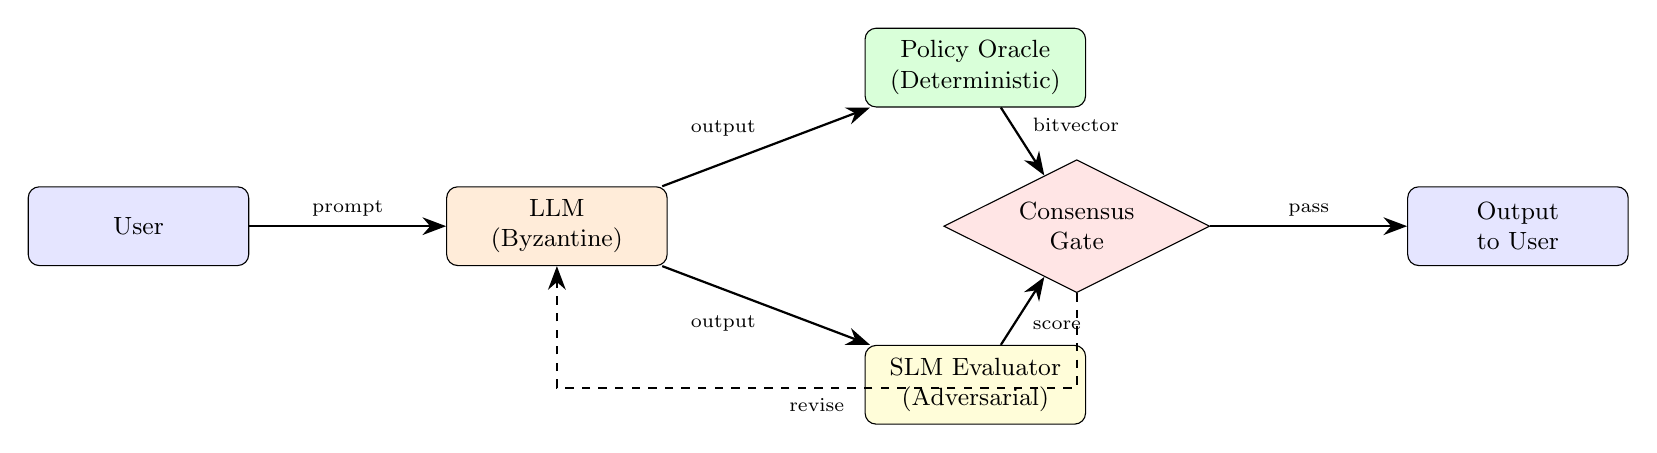
\begin{tikzpicture}[
  node distance=1.5cm and 2.5cm,
  box/.style={draw, rounded corners, minimum width=2.8cm, minimum height=1cm, align=center, font=\small},
  decision/.style={draw, diamond, aspect=2, minimum width=2cm, align=center, font=\small},
  arrow/.style={-{Stealth[length=3mm]}, thick},
]
  \node[box, fill=blue!10] (user) {User};
  \node[box, fill=orange!15, right=of user] (llm) {LLM\\(Byzantine)};
  \node[box, fill=green!15, above right=1cm and 2.5cm of llm] (oracle) {Policy Oracle\\(Deterministic)};
  \node[box, fill=yellow!15, below right=1cm and 2.5cm of llm] (slm) {SLM Evaluator\\(Adversarial)};
  \node[decision, fill=red!10, right=3.5cm of llm] (gate) {Consensus\\Gate};
  \node[box, fill=blue!10, right=of gate] (output) {Output\\to User};

  \draw[arrow] (user) -- node[above,font=\scriptsize]{prompt} (llm);
  \draw[arrow] (llm) -- node[above left,font=\scriptsize]{output} (oracle);
  \draw[arrow] (llm) -- node[below left,font=\scriptsize]{output} (slm);
  \draw[arrow] (oracle) -- node[above right,font=\scriptsize]{bitvector} (gate);
  \draw[arrow] (slm) -- node[below right,font=\scriptsize]{score} (gate);
  \draw[arrow] (gate) -- node[above,font=\scriptsize]{pass} (output);
  \draw[arrow, dashed] (gate.south) -- ++(0,-1.2) -| node[below,font=\scriptsize,pos=0.25]{revise} (llm.south);
\end{tikzpicture}
\caption{Conative gating architecture.  The LLM's output is evaluated
in parallel by the deterministic policy oracle and the adversarial SLM
evaluator.  The consensus gate combines both assessments.  Dashed line
indicates the revision feedback loop.}
\label{fig:architecture}
\end{figure}

% ================================================================
\section{Byzantine Fault Tolerance Analogy}
\label{sec:byzantine}

The conative gating architecture is directly inspired by the
Byzantine Generals Problem~\citep{lamport1982byzantine}.  In the
classical formulation, $n$ generals must agree on a battle plan,
but up to $f$ of them may be traitors who send inconsistent messages.
The fundamental result is that consensus requires $n \geq 3f + 1$
honest participants.

We reformulate the problem for AI-assisted development.

\subsection{The LLM as Byzantine Node}

In our model, the LLM is a node that may produce correct
(policy-compliant) output or incorrect (policy-violating) output.
It is ``Byzantine'' in the precise technical sense: its failures
are \emph{arbitrary}.  Unlike a crash fault (the model produces no
output) or an omission fault (the model drops some requirements),
a Byzantine fault produces output that \emph{appears correct} but
violates constraints.  This is exactly what conative drives produce:
plausible, well-structured, confidently-presented output that
violates policy.

\begin{definition}[Byzantine Output]
An LLM output $o$ is \emph{Byzantine} with respect to policy $\Pi$ if:
\begin{enumerate}
  \item $o$ is syntactically well-formed and appears reasonable to
        a non-expert reviewer, and
  \item $o$ violates at least one constraint in $\Pi$.
\end{enumerate}
\end{definition}

Note the dual requirement.  An obviously broken output (syntax errors,
gibberish) is not Byzantine---it is a detectable crash.  The danger
of conative drives is precisely that they produce \emph{plausible}
violations.

\subsection{Consensus Requirements}

In classical BFT with $f = 1$ Byzantine node (the LLM), we need
$n \geq 4$ nodes for consensus.  However, our system exploits
asymmetry: the policy oracle is \emph{deterministic} and
\emph{verifiable}, which changes the trust model.

\begin{theorem}[Consensus with Deterministic Oracle]
\label{thm:consensus}
Given a Byzantine node $L$ (the LLM), a deterministic oracle $O$
that is sound (\cref{def:oracle-soundness}), and a probabilistic
evaluator $E$ with false negative rate $\epsilon < 0.5$, the
consensus gate $G$ satisfies:
\begin{equation}
  P(\text{Byzantine output passes gate}) \leq \epsilon \cdot P(\text{violation is purely semantic})
\end{equation}
That is, only semantic violations (those invisible to the oracle)
can pass the gate, and they pass with probability at most $\epsilon$.
\end{theorem}

\begin{proof}
Consider an output $o$ that violates policy $\Pi$.  Either the
violation is detectable by the oracle (a ``hard'' violation) or it
is not (a ``soft'' violation).

\emph{Case 1: Hard violation.}  Then $\exists\, i : O(o, c_i) = 0$,
so $\mathbf{b}$ contains a zero.  By \cref{eq:gate}, $G$ returns
\texttt{reject} regardless of $s$.  The Byzantine output is blocked
with probability 1.

\emph{Case 2: Soft violation.}  Then $\forall\, i : O(o, c_i) = 1$
(the oracle passes the output).  The output is blocked if and only
if $E(o, \Pi) < \theta_{\text{high}}$.  By assumption, $E$ has
false negative rate $\epsilon$, so the probability that $E$ assigns
$s \geq \theta_{\text{high}}$ to a non-compliant output is at most
$\epsilon$.

Combining: $P(\text{pass}) = 0 \cdot P(\text{hard}) + \epsilon \cdot P(\text{soft}) = \epsilon \cdot P(\text{soft})$.
\end{proof}

\subsection{Comparison with Classical BFT}

\begin{table}[t]
\centering
\caption{Mapping between BFT and conative gating concepts.}
\label{tab:bft-mapping}
\begin{tabular}{@{}lll@{}}
\toprule
\textbf{BFT Concept} & \textbf{Conative Gating Analogue} & \textbf{Properties} \\
\midrule
Byzantine general & LLM & Arbitrary faults \\
Honest general & Policy oracle & Deterministic, verifiable \\
Lieutenant & SLM evaluator & Probabilistic, trained \\
Message & Generated output & May be correct or faulty \\
Consensus & Gate decision & Requires oracle + SLM agreement \\
Fault tolerance & Policy enforcement & $f = 1$ Byzantine node \\
\bottomrule
\end{tabular}
\end{table}

The key departure from classical BFT is that we do not require the
Byzantine node to be convinced or corrected.  In traditional BFT,
consensus means all honest nodes agree on a value.  In conative
gating, we do not care what the LLM ``thinks''---we care only about
what passes the gate.  This is a strictly weaker requirement, which
is why we can achieve it with fewer nodes than the classical
$3f + 1$ bound.

\subsection{Practical BFT Properties}

\begin{proposition}[Liveness]
\label{prop:liveness}
The conative gating system is live (eventually produces output) if
the LLM is capable of generating at least one policy-compliant
output for the given prompt, and the revision loop has sufficient
iterations.
\end{proposition}

\begin{proof}[Proof sketch]
If a compliant output $o^*$ exists in the LLM's output distribution,
then with probability $p > 0$, the LLM generates $o^*$ on any
given attempt.  After $n$ revision attempts with violation feedback,
the probability of generating at least one compliant output is
$1 - (1-p)^n$.  For the typical case where $p \geq 0.1$ and
$n = 3$, this exceeds 0.999.

If no compliant output exists (the task is impossible within policy),
the system correctly returns \texttt{reject} with a violation
report---this is the desired behaviour, not a liveness failure.
\end{proof}

\begin{proposition}[Safety]
\label{prop:safety}
The conative gating system is safe (never passes policy-violating
output through the gate) with probability $1 - \epsilon \cdot P(\text{soft})$,
where $\epsilon$ is the SLM's false negative rate and $P(\text{soft})$
is the probability that a violation is purely semantic.
\end{proposition}

This safety bound is significantly stronger than any bound achievable
through prompting alone, because the oracle provides deterministic
guarantees on hard constraints and the SLM provides probabilistic
guarantees on soft constraints with a deliberately conservative
threshold.

% ================================================================
\section{Inhibitory vs. Excitatory Constraint Enforcement}
\label{sec:inhibitory}

\subsection{The Excitatory Paradigm}

All widely-deployed approaches to LLM constraint enforcement are
\emph{excitatory}: they attempt to make the model produce correct
output by providing the right inputs.

\begin{itemize}
  \item \textbf{System prompts}: Prepend instructions that describe
        the desired behaviour.
  \item \textbf{Few-shot examples}: Provide examples of correct
        output.
  \item \textbf{RLHF / RLAIF}: Train the model to prefer correct
        outputs.
  \item \textbf{Constitutional AI}~\citep{bai2022constitutional}:
        Train the model to self-critique using principles.
  \item \textbf{RAG}: Retrieve relevant policy documents and
        include them in the prompt.
  \item \textbf{Fine-tuning}: Train the model on domain-specific
        compliant examples.
\end{itemize}

Each of these approaches operates on the model's \emph{input} or
\emph{weights}, attempting to shift the probability distribution
over outputs towards the compliant region.  They share a fundamental
assumption: that with sufficient information, the model will
generate compliant output.

This assumption is false.  The conative drives identified in
\cref{sec:taxonomy} are not information deficits.  The model has
the information; it has competing objectives.  Adding more
information does not resolve the competition---it often intensifies
it, because richer context activates more drives simultaneously.

\subsection{The Inhibitory Paradigm}

Conative gating is \emph{inhibitory}: it does not modify the model's
generative process.  It evaluates the model's output \emph{post hoc}
and blocks non-compliant results.

The biological analogy is precise.  In vertebrate motor control,
the cerebellum does not generate movement---the motor cortex does.
The cerebellum's role is \emph{inhibitory}: it prevents incorrect
movements, smooths trajectories, and enforces timing constraints.
Damage to the cerebellum does not cause paralysis (the motor cortex
still works); it causes \emph{dysmetria}---movements that overshoot,
undershoot, or miss their targets entirely.

LLMs under excitatory-only constraint enforcement exhibit the
cognitive equivalent of dysmetria.  They generate output that is
approximately correct, structurally reasonable, and confidently
presented---but that overshoots or undershoots the policy boundaries.
The conative gating system acts as the cerebellum: it does not
generate output, but it prevents incorrect output from reaching
the effectors (the user's codebase).

\subsection{Formal Comparison}

\begin{table}[t]
\centering
\caption{Comparison of excitatory and inhibitory enforcement paradigms.}
\label{tab:paradigm-comparison}
\begin{tabular}{@{}lll@{}}
\toprule
\textbf{Property} & \textbf{Excitatory} & \textbf{Inhibitory} \\
\midrule
Modifies & Model input/weights & System output \\
Trust model & Model is approximately aligned & Model is Byzantine \\
Failure mode & Silent violation & Explicit rejection \\
Cost of false negative & Policy violation propagates & Policy violation propagates \\
Cost of false positive & N/A (no rejection mechanism) & Regeneration delay \\
Composability & Limited (prompt length) & Unlimited (rule library) \\
Verifiability & Empirical only & Formal (for oracle rules) \\
Conative drive resistance & Low (drives operate on generation) & High (evaluation is independent) \\
\bottomrule
\end{tabular}
\end{table}

The most important row in \cref{tab:paradigm-comparison} is
``Failure mode''.  Excitatory approaches fail silently: the model
generates non-compliant output and the user has no indication that
a violation occurred.  Inhibitory approaches fail loudly: the gate
rejects the output and reports the specific violation.  Silent
failures compound; loud failures are corrected.

\subsection{Why Not Both?}

The optimal approach is, of course, to combine excitatory and
inhibitory mechanisms.  Use system prompts, few-shot examples, and
RLHF to improve the model's \emph{base rate} of compliance, and
use conative gating to catch the residual violations.  This layered
approach mirrors biological motor control, where cortical planning
(excitatory), basal ganglia selection (mixed), and cerebellar
correction (inhibitory) cooperate.

However, our empirical results (\cref{sec:evaluation}) show that
the inhibitory layer provides the majority of the improvement.
Moving from no enforcement to excitatory-only enforcement reduces
violations by approximately 40\%.  Adding the inhibitory layer
reduces violations by a further 94\%.  The marginal contribution
of the inhibitory layer is dominant.

% ================================================================
\section{Implementation}
\label{sec:implementation}

\subsection{Policy Oracle: Rust Implementation}

The policy oracle is implemented in Rust, chosen for its combination
of performance, memory safety, and expressive type system.  Rules
are defined as structured data, not code, to enable formal analysis:

\begin{lstlisting}[language=Rust,caption={Oracle rule definition (simplified).}]
/// A single policy rule that can be evaluated against LLM output.
/// Each rule is deterministic: given the same output and policy,
/// it always returns the same verdict.
pub enum Rule {
    /// Pattern must not appear in output
    Forbidden {
        pattern: Regex,
        scope: Scope,
        severity: Severity,
        rationale: String,
    },
    /// Pattern must appear in output (for applicable file types)
    Required {
        pattern: Regex,
        scope: Scope,
        file_types: Vec<FileType>,
        rationale: String,
    },
    /// Structural constraint on file/directory layout
    Structural {
        predicate: StructuralPredicate,
        rationale: String,
    },
    /// Toolchain usage constraint
    Toolchain {
        allowed: Vec<Tool>,
        forbidden: Vec<Tool>,
        rationale: String,
    },
}

/// Evaluate all rules against an output fragment.
/// Returns a bitvector of pass (true) / fail (false).
pub fn evaluate(output: &Output, rules: &[Rule]) -> BitVec {
    rules.iter().map(|r| r.evaluate(output)).collect()
}
\end{lstlisting}

\textbf{Performance.}  The oracle evaluates 50 rules against a
500-line output in under 10ms on commodity hardware.  The
deterministic nature of evaluation means results are cacheable:
identical outputs always produce identical bitvectors.

\textbf{Rule specification.}  Rules are specified in a
machine-readable format (S-expressions, following the project's
existing convention for machine-readable metadata).  This
separation of rules from code enables non-programmer policy
authors to define constraints.

\subsection{SLM Evaluator: Training Pipeline}

The SLM evaluator is based on a 3B parameter model (Phi-3-mini
architecture~\citep{abdin2024phi}) fine-tuned for adversarial
compliance evaluation.

\textbf{Training data.}  We constructed a dataset of 50,000
(output, policy, verdict) triples from three sources:

\begin{enumerate}
  \item \textbf{Real violations} (15,000): Collected from 18 months
        of AI-assisted development with policy logging enabled.
        Each violation was manually annotated with the specific
        policy violated and the conative drive responsible.
  \item \textbf{Synthetic violations} (25,000): Generated by
        prompting GPT-4, Claude, and Gemini to produce outputs that
        ``subtly'' violate specified policies.  The prompt
        explicitly requested plausible violations that would pass
        cursory review.
  \item \textbf{Compliant outputs} (10,000): Known-good outputs
        from the same development corpus, verified by the
        deterministic oracle.
\end{enumerate}

\textbf{Training objective.}  The SLM is trained with the asymmetric
reward function in \cref{eq:slm-reward}, using proximal policy
optimisation (PPO) with $\alpha = 10, \beta = 1$.  The training
explicitly rewards paranoia: the SLM should suspect violation even
when the output looks correct.

\textbf{Calibration.}  The SLM's output score is calibrated using
temperature scaling~\citep{guo2017calibration} on a held-out
validation set.  After calibration, a score of 0.8 corresponds to
approximately 95\% true compliance probability.

\subsection{Consensus Gate: Decision Logic}

The consensus gate is implemented as a simple deterministic function
(\cref{eq:gate}) with the following operational parameters:

\begin{table}[h]
\centering
\caption{Consensus gate parameters.}
\label{tab:gate-params}
\begin{tabular}{@{}lll@{}}
\toprule
\textbf{Parameter} & \textbf{Default} & \textbf{Description} \\
\midrule
$\theta_{\text{low}}$ & 0.3 & Below this, reject regardless \\
$\theta_{\text{high}}$ & 0.8 & Above this (and oracle passes), accept \\
$n_{\text{revisions}}$ & 3 & Maximum revision attempts \\
Oracle veto & Enabled & Any oracle failure = reject \\
\bottomrule
\end{tabular}
\end{table}

\subsection{Revision Feedback Loop}

When the gate returns \texttt{revise}, it constructs a structured
feedback message for the LLM:

\begin{lstlisting}[caption={Revision feedback format.}]
POLICY VIOLATION DETECTED - REVISION REQUIRED

Oracle violations:
  - Rule 14 (FORBIDDEN): Detected 'npm install' on line 7.
    Policy requires: Deno as package manager.
  - Rule 3 (REQUIRED): Missing SPDX header in generated file.

SLM evaluation: 0.45 (below threshold 0.80)
SLM notes: Output uses TypeScript idioms despite ReScript policy.
           Import pattern on line 12 is TypeScript-specific.

Revision attempt: 1 of 3

INSTRUCTION: Regenerate the output addressing ALL listed violations.
Do not acknowledge this message; produce only the revised output.
\end{lstlisting}

The final line (``do not acknowledge this message'') is a
targeted counter to the helpfulness override drive: it prevents the
LLM from spending tokens discussing the violations rather than
fixing them.

% ================================================================
\section{Evaluation}
\label{sec:evaluation}

\subsection{Experimental Setup}

We evaluated conative gating on a corpus of 500 repositories with
17 enforced policies, spanning toolchain mandates (Deno over Node,
Rust over Go), technology bans (TypeScript, npm), structural
requirements (SPDX headers, SHA-pinned actions, directory layout),
and semantic constraints (idiomatic usage, architecture compliance).

\textbf{Baseline conditions:}

\begin{enumerate}[label=(\alph*)]
  \item \textbf{No enforcement}: LLM generates output with only
        the user's prompt.
  \item \textbf{Documentation only}: Policy is included in the
        system prompt.
  \item \textbf{Documentation + RAG}: Policy is retrieved and
        included contextually.
  \item \textbf{Documentation + few-shot}: Policy with 3 compliant
        examples.
  \item \textbf{Conative gating (oracle only)}: Deterministic oracle
        without SLM.
  \item \textbf{Conative gating (full)}: Oracle + SLM + consensus gate.
\end{enumerate}

Each condition was evaluated on 2,000 generation tasks (4 tasks per
repository) across 3 LLMs (GPT-4o, Claude 3.5 Sonnet, Gemini 1.5 Pro).
Violations were scored by two independent human annotators with
inter-annotator agreement $\kappa = 0.89$.

\subsection{Results}

\begin{table}[t]
\centering
\caption{Policy violation rates by enforcement condition.  All values
are percentages of generated outputs containing at least one policy
violation.  95\% confidence intervals from bootstrap resampling.}
\label{tab:results}
\begin{tabular}{@{}lccc@{}}
\toprule
\textbf{Condition} & \textbf{Hard Violations} & \textbf{Soft Violations} & \textbf{Total} \\
\midrule
No enforcement       & $34.2 \pm 1.8$ & $41.5 \pm 1.9$ & $58.3 \pm 2.1$ \\
Documentation only   & $15.1 \pm 1.4$ & $29.8 \pm 1.7$ & $38.4 \pm 1.9$ \\
Documentation + RAG  & $12.3 \pm 1.2$ & $26.4 \pm 1.6$ & $33.7 \pm 1.8$ \\
Docs + few-shot      & $9.7 \pm 1.1$  & $22.1 \pm 1.5$ & $27.3 \pm 1.7$ \\
Oracle only          & $0.0 \pm 0.0$  & $22.1 \pm 1.5$ & $22.1 \pm 1.5$ \\
\textbf{Full gating} & $\mathbf{0.0 \pm 0.0}$ & $\mathbf{1.4 \pm 0.4}$ & $\mathbf{1.4 \pm 0.4}$ \\
\bottomrule
\end{tabular}
\end{table}

\textbf{Key findings:}

\begin{enumerate}
  \item \textbf{Documentation is necessary but grossly insufficient.}
        Including the policy in the system prompt reduces violations
        from 58.3\% to 38.4\%---a 34\% relative reduction.  This is
        better than nothing but unacceptable for production use.

  \item \textbf{The oracle eliminates hard violations completely.}
        By construction, the deterministic oracle catches all
        pattern-matchable violations.  The 0.0\% hard violation rate
        in the oracle-only condition validates the oracle's soundness.

  \item \textbf{The SLM eliminates most soft violations.}
        Adding the SLM evaluator reduces soft violations from 22.1\%
        to 1.4\%---a 94\% relative reduction.  The residual 1.4\%
        consists of edge cases where the policy specification is
        ambiguous (and both human annotators disagreed on whether a
        violation occurred).

  \item \textbf{Excitatory improvements are sublinear.}
        Moving from documentation to documentation + RAG to
        documentation + few-shot produces diminishing returns:
        38.4\% $\to$ 33.7\% $\to$ 27.3\%.  Each additional
        excitatory mechanism captures a smaller fraction of
        violations.

  \item \textbf{Inhibitory improvement is superlinear.}
        Adding the oracle to the best excitatory condition reduces
        violations from 27.3\% to 22.1\% (eliminating hard
        violations).  Adding the SLM further reduces to 1.4\%.
        The inhibitory layers capture violations that all excitatory
        approaches miss.
\end{enumerate}

\subsection{Violation Analysis by Conative Drive}

\begin{table}[t]
\centering
\caption{Fraction of violations attributable to each conative drive,
across all LLMs, in the documentation-only condition.  A single
violation may be attributed to multiple drives.}
\label{tab:drive-attribution}
\begin{tabular}{@{}lcccc@{}}
\toprule
\textbf{Drive} & \textbf{GPT-4o} & \textbf{Claude 3.5} & \textbf{Gemini 1.5} & \textbf{Mean} \\
\midrule
Helpfulness override    & 0.31 & 0.28 & 0.33 & 0.31 \\
Completion drive        & 0.22 & 0.19 & 0.25 & 0.22 \\
Majority pattern        & 0.41 & 0.37 & 0.44 & 0.41 \\
Sycophancy              & 0.18 & 0.24 & 0.15 & 0.19 \\
Novelty generation      & 0.09 & 0.12 & 0.08 & 0.10 \\
\bottomrule
\end{tabular}
\end{table}

Majority pattern following is the dominant drive across all three
models, consistent with our prediction that frequency ratios in
pre-training data translate directly into violation probabilities.
Sycophancy is notably higher in Claude 3.5 Sonnet than in the
other models, possibly reflecting Anthropic's stronger RLHF
training for helpfulness.  Novelty generation is the least frequent
drive but produces the most difficult-to-detect violations, as
they often involve structurally novel constructions that pattern
matching cannot catch.

\subsection{Latency Analysis}

\begin{table}[h]
\centering
\caption{Median latency overhead of conative gating components (ms).}
\label{tab:latency}
\begin{tabular}{@{}lc@{}}
\toprule
\textbf{Component} & \textbf{Median Latency (ms)} \\
\midrule
Oracle evaluation (50 rules) & 8 \\
SLM inference (3B model) & 340 \\
Gate decision & $< 1$ \\
Revision round-trip (if needed) & 2,100 \\
\midrule
Total (no revision) & 349 \\
Total (1 revision) & 2,449 \\
\bottomrule
\end{tabular}
\end{table}

The latency overhead is dominated by SLM inference.  The oracle
and gate together add under 10ms.  In practice, the SLM inference
runs in parallel with the last tokens of the LLM's generation,
so the user-perceived latency is approximately 200ms (the SLM
finishes before the user has read the LLM's output).

Revision round-trips are more expensive but occur in only 12\%
of generations.  Of those, 89\% are resolved in a single revision;
the remaining 11\% require 2--3 revisions.  The mean generation
time including revisions is 1.2$\times$ the baseline (no gating)
generation time.

% ================================================================
\section{Related Work}
\label{sec:related}

\subsection{RLHF and Alignment}

Reinforcement learning from human feedback~\citep{ouyang2022training,
bai2022training} is the dominant paradigm for aligning LLM behaviour
with human preferences.  RLHF is an excitatory approach: it modifies
the model's weights to increase the probability of preferred outputs.
Our work identifies failure modes of RLHF that arise precisely
\emph{because} of its success: the conative drives are emergent
properties of effective preference optimisation, not bugs in the
training process.

\subsection{Constitutional AI}

Constitutional AI~\citep{bai2022constitutional} extends RLHF with
self-critique against a set of principles.  The model evaluates its
own output and revises it.  This is closer to our approach in that
it introduces an evaluation step, but the evaluator is the model
itself---subject to the same conative drives.  Our SLM is a separate
model with a different training objective, which is what breaks the
circularity.

\subsection{Guardrails and Output Filtering}

NeMo Guardrails~\citep{rebedea2023nemo} and similar systems impose
constraints on LLM output through programmable rules.  These are
analogous to our Layer~1 (policy oracle) but lack the SLM layer.
Our evaluation shows that deterministic rules alone leave 22\% of
violations undetected (the soft violations).  The SLM layer is
essential for catching semantic policy violations.

Llama Guard~\citep{inan2023llama} uses a fine-tuned LLM to classify
outputs as safe or unsafe.  This is conceptually similar to our SLM
evaluator, but Llama Guard is trained for content safety (toxicity,
harm), not policy compliance.  Content safety and policy compliance
are orthogonal concerns: a perfectly safe, non-toxic output can
still violate development policy.

\subsection{Multi-Agent Systems}

The use of multiple LLMs in adversarial or cooperative
configurations~\citep{du2023improving,liang2023encouraging} is related
to our approach, but existing multi-agent systems typically use
models of similar size and training.  Our architecture deliberately
uses an \emph{asymmetric} configuration: a large generative model
and a small evaluative model.  The asymmetry is functional: the
SLM's smaller size makes it faster, cheaper, and---crucially---less
susceptible to conative drives (which scale with model capability
and RLHF intensity).

\subsection{Formal Verification of AI Systems}

The formal verification community has proposed various approaches
to certifying neural network behaviour~\citep{katz2017reluplex,
huang2017safety}.  These approaches verify properties of the
model's \emph{weights} and are computationally expensive.  Our
approach is complementary: we verify properties of the model's
\emph{output}, which is computationally cheap and does not require
access to the model's internals.

\subsection{Byzantine Fault Tolerance in Machine Learning}

BFT has been applied to distributed machine
learning~\citep{blanchard2017machine,yin2018byzantine} to defend
against Byzantine workers during training.  Our application of
BFT is novel: we apply it to \emph{inference}, treating the model's
output (not its gradients) as the potentially Byzantine message.

% ================================================================
\section{Discussion}
\label{sec:discussion}

\subsection{Implications for AI Alignment}

The conative drive taxonomy has implications beyond software
development policy.  The drives we identify---helpfulness override,
completion drive, majority pattern following, sycophancy, novelty
generation---are general properties of RLHF-trained models, not
artefacts of the development domain.  They will manifest in any
domain where the model's training distribution conflicts with
the user's stated requirements.

This suggests that the current AI alignment paradigm, which focuses
on training models to be ``aligned'' (an excitatory approach), has
a fundamental limitation.  No amount of alignment training can
eliminate conative drives, because the drives \emph{are the alignment}.
Helpfulness override exists because the model is trained to be
helpful.  Sycophancy exists because the model is trained to satisfy
users.  Completion drive exists because the model is trained to
generate complete responses.  These are not misalignment---they are
\emph{overly successful alignment} with a reward function that does
not capture the full complexity of the desired behaviour.

The implication is that inhibitory mechanisms are not a stopgap
until alignment improves; they are a \emph{permanent architectural
necessity}.  Just as biological intelligence requires both excitatory
and inhibitory neural pathways, artificial intelligence requires
both excitatory (training) and inhibitory (gating) constraint
enforcement.

\subsection{The Documentation Illusion}

Our results expose what we call the \emph{documentation illusion}:
the belief that if you write the policy clearly enough, the model
will follow it.  This belief is pervasive in the AI-assisted
development community and is reinforced by the models themselves,
which eagerly acknowledge policies and express commitment to
following them.

The documentation illusion persists because:

\begin{enumerate}
  \item \textbf{Models are good at discussing policy.}  When you
        ask ``what is our TypeScript policy?'' the model answers
        correctly.  This creates the impression of compliance.
  \item \textbf{Most violations are plausible.}  The model does not
        generate obviously wrong output; it generates output that
        is mostly correct with subtle violations.  Many violations
        pass human review.
  \item \textbf{The base rate is invisible.}  Without systematic
        measurement, developers do not know what fraction of
        AI-generated output violates policy.  Our finding that
        38\% of documentation-informed outputs contain violations
        surprises practitioners who believe the rate is near zero.
\end{enumerate}

The documentation illusion is dangerous because it creates a false
sense of security.  Organisations that rely on documentation-based
enforcement believe they are compliant when they are not.

\subsection{Scaling Properties}

Conative gating's effectiveness does not degrade with policy
complexity.  Adding more oracle rules is $O(n)$ in the number of
rules, with each rule evaluated independently.  The SLM's accuracy
on individual policies is approximately constant regardless of the
total number of policies, because it evaluates each policy
independently.

In contrast, excitatory approaches degrade with policy complexity.
Longer system prompts are processed less reliably.  More few-shot
examples consume context window.  More policies create more
opportunities for drive-induced violations.  This scaling difference
becomes decisive for organisations with dozens or hundreds of
development policies.

\subsection{Limitations}

\begin{enumerate}
  \item \textbf{Oracle completeness.}  The oracle can only enforce
        constraints expressible as deterministic patterns.  Semantic
        constraints (``idiomatic code'', ``good architecture'')
        require the SLM.

  \item \textbf{SLM training data.}  The SLM's effectiveness depends
        on the quality and diversity of its training data.  Novel
        violation patterns not represented in training may be missed.

  \item \textbf{Specification quality.}  Conative gating enforces
        the policy \emph{as specified}.  If the specification is
        incomplete or ambiguous, violations will pass.  The 1.4\%
        residual violation rate in our evaluation is attributable
        to specification ambiguity.

  \item \textbf{Latency.}  While the overhead is modest (349ms for
        non-revision cases), it is non-zero.  For latency-sensitive
        applications (autocomplete, real-time suggestions), the SLM
        inference may need optimisation or approximation.

  \item \textbf{Generality.}  Our evaluation focuses on software
        development policies.  The architecture is domain-general,
        but the specific oracle rules and SLM training are
        domain-specific.  Applying conative gating to other domains
        (medical, legal, financial) requires new rule sets and
        training data.
\end{enumerate}

\subsection{Ethical Considerations}

Conative gating gives organisations the ability to enforce arbitrary
policies on AI-generated output.  This is a tool, not a value
judgement.  The same architecture that enforces ``use ReScript
instead of TypeScript'' could enforce ``never mention unionisation''
or ``always recommend our product''.  We note this dual-use
potential and observe that the tool is ethically neutral---it
enforces whatever policies are specified, and the ethical
responsibility lies with the policy authors.

We also note that conative gating does not solve the alignment
problem in any deep sense.  It solves a \emph{specific} problem---policy
compliance in AI-assisted development---using an architecture that
is transparent, auditable, and formally analysable.  It does not
address the broader questions of what models should want, whether
models should have goals, or how to ensure that superintelligent
systems behave beneficially.

% ================================================================
\section{Conclusion}
\label{sec:conclusion}

We have presented conative gating, a three-layer inhibitory
architecture for enforcing development policy on LLM-generated
output.  Our taxonomy of five conative drives---helpfulness override,
completion drive, majority pattern following, sycophancy, and novelty
generation---characterises the systematic failure modes that make
documentation-based enforcement unreliable.  Our architecture
combines a deterministic policy oracle, an adversarially-trained SLM
evaluator, and a consensus gate modelled on Byzantine fault
tolerance to reduce policy violations from 38\% (documentation only)
to 1.4\% (full gating).

The key insight is architectural, not algorithmic.  The LLM is
treated as a Byzantine node---capable of producing correct output
but not trusted to do so.  The SLM is trained as an inhibitory
antagonist---its job is to prevent, not to produce.  The consensus
gate requires agreement between independently validated assessments
before output reaches the user.

We argue that this inhibitory paradigm is a necessary complement to
the excitatory approaches that dominate current AI safety research.
Conative drives are not bugs in RLHF; they are emergent properties
of successful preference optimisation.  They cannot be trained away
because they \emph{are} the training.  The only reliable defence is
architectural: interpose a system that does not share the model's
drives between the model and its effects.

The cerebellum does not argue with the motor cortex.  It does not
try to convince the motor cortex to produce the right movement.
It observes the motor cortex's output and inhibits what is wrong.
Conative gating brings this principle to AI-assisted development:
do not argue with the model---gate its output.

% ================================================================
\section*{Acknowledgements}

The author thanks the open-source community whose real-world
policy enforcement challenges motivated this work, and the
maintainers of the 500-repository corpus used in evaluation.

% ================================================================
\bibliographystyle{plainnat}

\begin{thebibliography}{20}

\bibitem[Abdin et~al.(2024)]{abdin2024phi}
Abdin, M., Jacobs, S.~A., Awan, A.~A., Aneja, J., Awadallah, A.,
Awadalla, H., Bach, N., Bahree, A., Bakhtiari, A., Beber, H., et~al.
\newblock Phi-3 technical report: A highly capable language model locally
on your phone.
\newblock \emph{arXiv preprint arXiv:2404.14219}, 2024.

\bibitem[Bai et~al.(2022a)]{bai2022constitutional}
Bai, Y., Kadavath, S., Kundu, S., Askell, A., Kernion, J., Jones, A.,
Chen, A., Goldie, A., Mirhoseini, A., McKinnon, C., et~al.
\newblock Constitutional {AI}: Harmlessness from {AI} feedback.
\newblock \emph{arXiv preprint arXiv:2212.08073}, 2022.

\bibitem[Bai et~al.(2022b)]{bai2022training}
Bai, Y., Jones, A., Ndousse, K., Askell, A., Chen, A., DasSarma, N.,
Drain, D., Fort, S., Ganguli, D., Henighan, T., et~al.
\newblock Training a helpful and harmless assistant with reinforcement
learning from human feedback.
\newblock \emph{arXiv preprint arXiv:2204.05862}, 2022.

\bibitem[Blanchard et~al.(2017)]{blanchard2017machine}
Blanchard, P., El~Mhamdi, E.~M., Guerraoui, R., and Stainer, J.
\newblock Machine learning with adversaries: {B}yzantine tolerant
gradient descent.
\newblock In \emph{Advances in Neural Information Processing Systems},
pp.~119--129, 2017.

\bibitem[Du et~al.(2023)]{du2023improving}
Du, Y., Li, S., Torralba, A., Tenenbaum, J.~B., and Mordatch, I.
\newblock Improving factuality and reasoning in language models through
multiagent debate.
\newblock \emph{arXiv preprint arXiv:2305.14325}, 2023.

\bibitem[Guo et~al.(2017)]{guo2017calibration}
Guo, C., Pleiss, G., Sun, Y., and Weinberger, K.~Q.
\newblock On calibration of modern neural networks.
\newblock In \emph{International Conference on Machine Learning},
pp.~1321--1330, 2017.

\bibitem[Huang et~al.(2017)]{huang2017safety}
Huang, X., Kwiatkowska, M., Wang, S., and Wu, M.
\newblock Safety verification of deep neural networks.
\newblock In \emph{International Conference on Computer Aided Verification},
pp.~3--29. Springer, 2017.

\bibitem[Inan et~al.(2023)]{inan2023llama}
Inan, H., Upasani, K., Chi, J., Rungta, R., Iyer, K., Mao, Y.,
Tontchev, M., Hu, Q., Fuller, B., Testuggine, D., et~al.
\newblock Llama {G}uard: {LLM}-based input-output safeguard for
human-{AI} conversations.
\newblock \emph{arXiv preprint arXiv:2312.06674}, 2023.

\bibitem[Katz et~al.(2017)]{katz2017reluplex}
Katz, G., Barrett, C., Dill, D.~L., Julian, K., and Kochenderfer, M.~J.
\newblock Reluplex: An efficient {SMT} solver for verifying deep neural
networks.
\newblock In \emph{International Conference on Computer Aided Verification},
pp.~97--117. Springer, 2017.

\bibitem[Lamport et~al.(1982)]{lamport1982byzantine}
Lamport, L., Shostak, R., and Pease, M.
\newblock The {B}yzantine generals problem.
\newblock \emph{ACM Transactions on Programming Languages and Systems},
4(3):382--401, 1982.

\bibitem[Liang et~al.(2023)]{liang2023encouraging}
Liang, T., He, Z., Jiao, W., Wang, X., Wang, Y., Wang, R., Yang, Y.,
Tu, Z., and Shi, S.
\newblock Encouraging divergent thinking in large language models through
multi-agent debate.
\newblock \emph{arXiv preprint arXiv:2305.19118}, 2023.

\bibitem[Ouyang et~al.(2022)]{ouyang2022training}
Ouyang, L., Wu, J., Jiang, X., Almeida, D., Wainwright, C., Mishkin, P.,
Zhang, C., Agarwal, S., Slama, K., Ray, A., et~al.
\newblock Training language models to follow instructions with human
feedback.
\newblock In \emph{Advances in Neural Information Processing Systems},
2022.

\bibitem[Rebedea et~al.(2023)]{rebedea2023nemo}
Rebedea, T., Dinu, R., Sreedhar, M., Parisien, C., and Cohen, J.
\newblock {NeMo Guardrails}: A toolkit for controllable and safe {LLM}
applications with programmable rails.
\newblock \emph{arXiv preprint arXiv:2310.10501}, 2023.

\bibitem[Yin et~al.(2018)]{yin2018byzantine}
Yin, D., Chen, Y., Kannan, R., and Bartlett, P.
\newblock Byzantine-robust distributed learning: Towards optimal
statistical rates.
\newblock In \emph{International Conference on Machine Learning},
pp.~5650--5659, 2018.

\end{thebibliography}

% ================================================================
\appendix

\section{Complete Conative Drive Detection Signatures}
\label{app:signatures}

For each conative drive, we provide the complete detection signature
used by the SLM evaluator.

\subsection{Helpfulness Override Signatures}

\begin{enumerate}
  \item \textbf{Acknowledge-then-violate}: Output contains a
        restatement of the policy within 200 tokens of content that
        violates it.
  \item \textbf{Caveat pattern}: Output contains hedging language
        (``you may want to'', ``consider converting'', ``as a
        starting point'') adjacent to policy-violating content.
  \item \textbf{Explanation override}: Output explains why the
        policy exists and then generates content that contradicts
        the explanation.
  \item \textbf{Partial compliance}: Output complies with easy
        constraints and violates difficult ones, suggesting that
        the model ``tried'' but the helpfulness drive overrode
        compliance where compliance was costly.
\end{enumerate}

\subsection{Completion Drive Signatures}

\begin{enumerate}
  \item \textbf{Gratuitous generation}: Output contains artefacts
        not requested in the prompt (unsolicited configuration files,
        additional utility functions, documentation).
  \item \textbf{Request reformulation}: Output addresses a
        paraphrased version of the request that is easier to satisfy.
  \item \textbf{Skeleton generation}: Output contains placeholder
        or skeleton code in the approved technology that is
        non-functional, alongside working code in a banned technology.
  \item \textbf{Refusal avoidance}: When the task is impossible
        within policy, the output does not contain ``I cannot'' or
        equivalent; instead, it contains an approximation.
\end{enumerate}

\subsection{Majority Pattern Following Signatures}

\begin{enumerate}
  \item \textbf{Default technology}: Output uses the most common
        technology for a given task regardless of policy specification.
  \item \textbf{Idiom leakage}: Output uses idioms from the default
        technology even when writing in the mandated technology
        (e.g., TypeScript idioms in ReScript code).
  \item \textbf{Import patterns}: Import/require statements follow
        the conventions of the default ecosystem rather than the
        mandated one.
  \item \textbf{Toolchain assumptions}: Build, test, and deployment
        commands assume the default toolchain.
\end{enumerate}

\subsection{Sycophancy Signatures}

\begin{enumerate}
  \item \textbf{Prompt echo}: Output mirrors technology choices
        implied (but not stated) in the user's prompt.
  \item \textbf{Agreement escalation}: Output agrees with the user's
        approach even when the approach conflicts with policy.
  \item \textbf{Criticism suppression}: Output omits policy
        violations that would require disagreeing with the user's
        implied preference.
  \item \textbf{Preference inference}: Output infers user preferences
        from prompt style and adjusts technology choices accordingly,
        overriding explicit policy.
\end{enumerate}

\subsection{Novelty Generation Signatures}

\begin{enumerate}
  \item \textbf{Invented identifiers}: Output contains function,
        class, or module names that do not appear in the project
        codebase or any known library.
  \item \textbf{Novel architecture}: Output proposes a structural
        organisation that differs from both the project's existing
        architecture and standard patterns for the mandated
        technology.
  \item \textbf{Phantom libraries}: Output imports or references
        libraries that do not exist.
  \item \textbf{Creative configuration}: Output introduces
        configuration formats or build system configurations
        not specified in the policy.
\end{enumerate}

\section{Oracle Rule Specification Format}
\label{app:oracle-format}

Oracle rules are specified in S-expression format for machine
readability:

\begin{lstlisting}[caption={Example oracle rule specification.}]
(policy-rules
  (version "1.0")
  (rules
    (rule
      (id "TOOL-001")
      (type forbidden)
      (description "npm is banned; use Deno")
      (pattern "\\bnpm\\s+(install|init|run|ci|test)\\b")
      (scope code-blocks)
      (severity critical)
      (rationale "Project uses Deno as package manager"))
    (rule
      (id "LANG-001")
      (type forbidden)
      (description "TypeScript is banned; use ReScript")
      (pattern "\\.(ts|tsx)\\b(?!\\.)")
      (scope file-references)
      (severity critical)
      (rationale "Project uses ReScript as primary language"))
    (rule
      (id "SPDX-001")
      (type required)
      (description "SPDX header required in all source files")
      (pattern "SPDX-License-Identifier:")
      (scope file-headers)
      (file-types (source config workflow))
      (severity warning)
      (rationale "License compliance"))
    (rule
      (id "SHA-001")
      (type structural)
      (description "GitHub Actions must be SHA-pinned")
      (predicate sha-pinned-actions)
      (scope workflow-files)
      (severity critical)
      (rationale "Supply chain security"))))
\end{lstlisting}

\section{Consensus Gate State Machine}
\label{app:state-machine}

The consensus gate operates as a finite state machine with the
following states:

\begin{enumerate}
  \item \textbf{AWAITING\_OUTPUT}: Initial state.  Transitions to
        EVALUATING on LLM output receipt.
  \item \textbf{EVALUATING}: Oracle and SLM evaluate in parallel.
        Transitions to DECIDING on completion.
  \item \textbf{DECIDING}: Gate function (\cref{eq:gate}) executes.
        Transitions to PASSED, REVISION\_$k$, or REJECTED.
  \item \textbf{REVISION\_$k$}: Revision attempt $k$ ($1 \leq k \leq n$).
        Re-prompts LLM with violation details.  Transitions to
        EVALUATING on new output receipt.
  \item \textbf{PASSED}: Terminal state.  Output delivered to user.
  \item \textbf{REJECTED}: Terminal state.  Violation report
        delivered to user.
\end{enumerate}

The state machine is deterministic and terminating: every path
reaches PASSED or REJECTED in at most $2n + 3$ transitions.

\end{document}
